\subsection{Clustering accuracy} \label{integr-synth-cluster-sect}
Evaluation of the \emph{clustering accuracy} for the BCC model will be made on the same 100 realizations of the synthetic data that were used for evaluating the accuracy of the adherence parameter.

The metrics considered are the source-specific and overall clustering errors, $\mathbf{L}_{error}$ and $\mathbf{C}_{error}$ respectively, which compute the average number of incorrect cluster assignments. 
\begin{equation}
  \begin{aligned}
  	\mathbf{L}_{error} & = \frac{\sum\limits_{m=1}^{M}\sum\limits_{n=1}^{N}\mathbbm{1}(\hat{L}_{mn} \neq L_{mn})}{MN} \\
  	\mathbf{C}_{error} & = \frac{\sum\limits_{n=1}^{n}\mathbbm{1}(\hat{C}_{n} \neq C_{n})}{N}
  \end{aligned}
\end{equation}
where $\hat{L}_{mn}, \hat{C}_{n}$ denote the estimated source-specific and overall clustering assignments, and $\mathbbm{1}(\cdot)$ is the indicator function.

The relative error for the source-specific and the overall clusterings is shown in \emph{Fig. \ref{source-error-pic}} and \emph{Fig. \ref{overall-error-pic}}, respectively. The results in each figure are shown as a function of $\alpha$. \emph{LOESS} regression \citep{Cleveland1979} is fit to the results so as to produce smooth curves. Care should be taken when comparing the results between the two figures, since the y-axis limits for $\mathbf{L}_{error}$ are $(0,0.12)$, whereas for $\mathbf{C}_{error}$ are $(0,0.52)$. This difference is not surprising, since the clustering problem is much easier when performed on each data source individually, especially for our synthetic data where the different clusters are well separated. 
\begin{figure}[!ht]
\begin{center}
 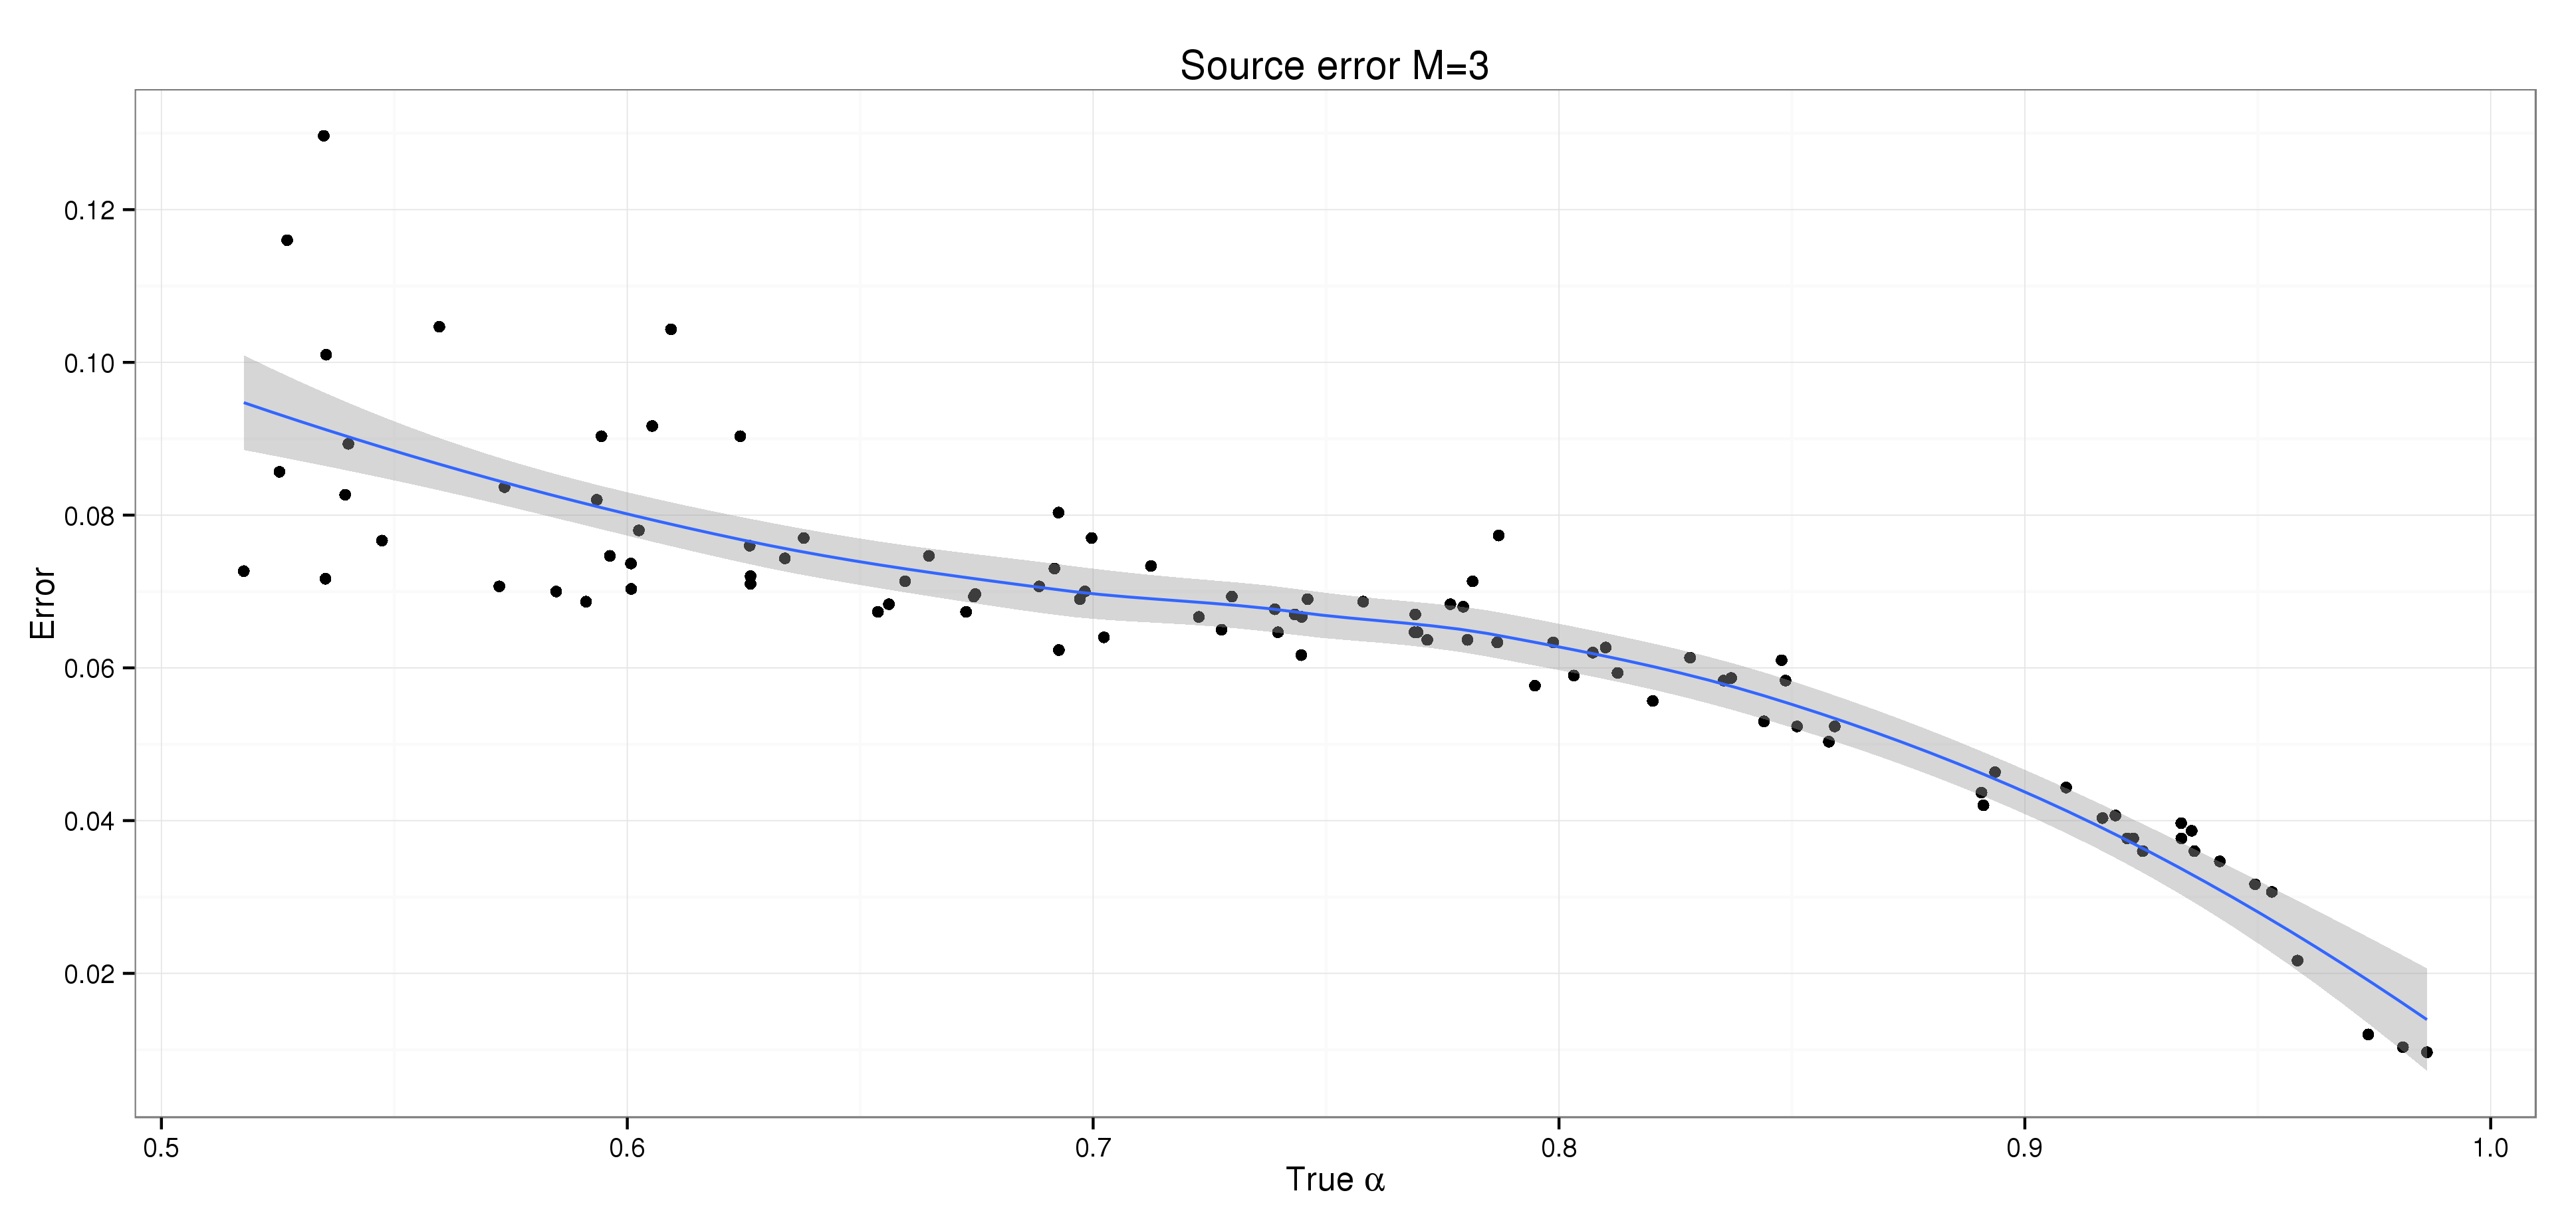
\includegraphics[scale = 0.39]{images/sourceError.png}
\caption{\emph{Source-specific clustering error as a function of $\alpha$ for 100 realizations with $M=3$ data sources and $K=2$ clusters.}}
\label{source-error-pic}
\end{center}
\end{figure}

\begin{figure}[!ht]
\begin{center}
 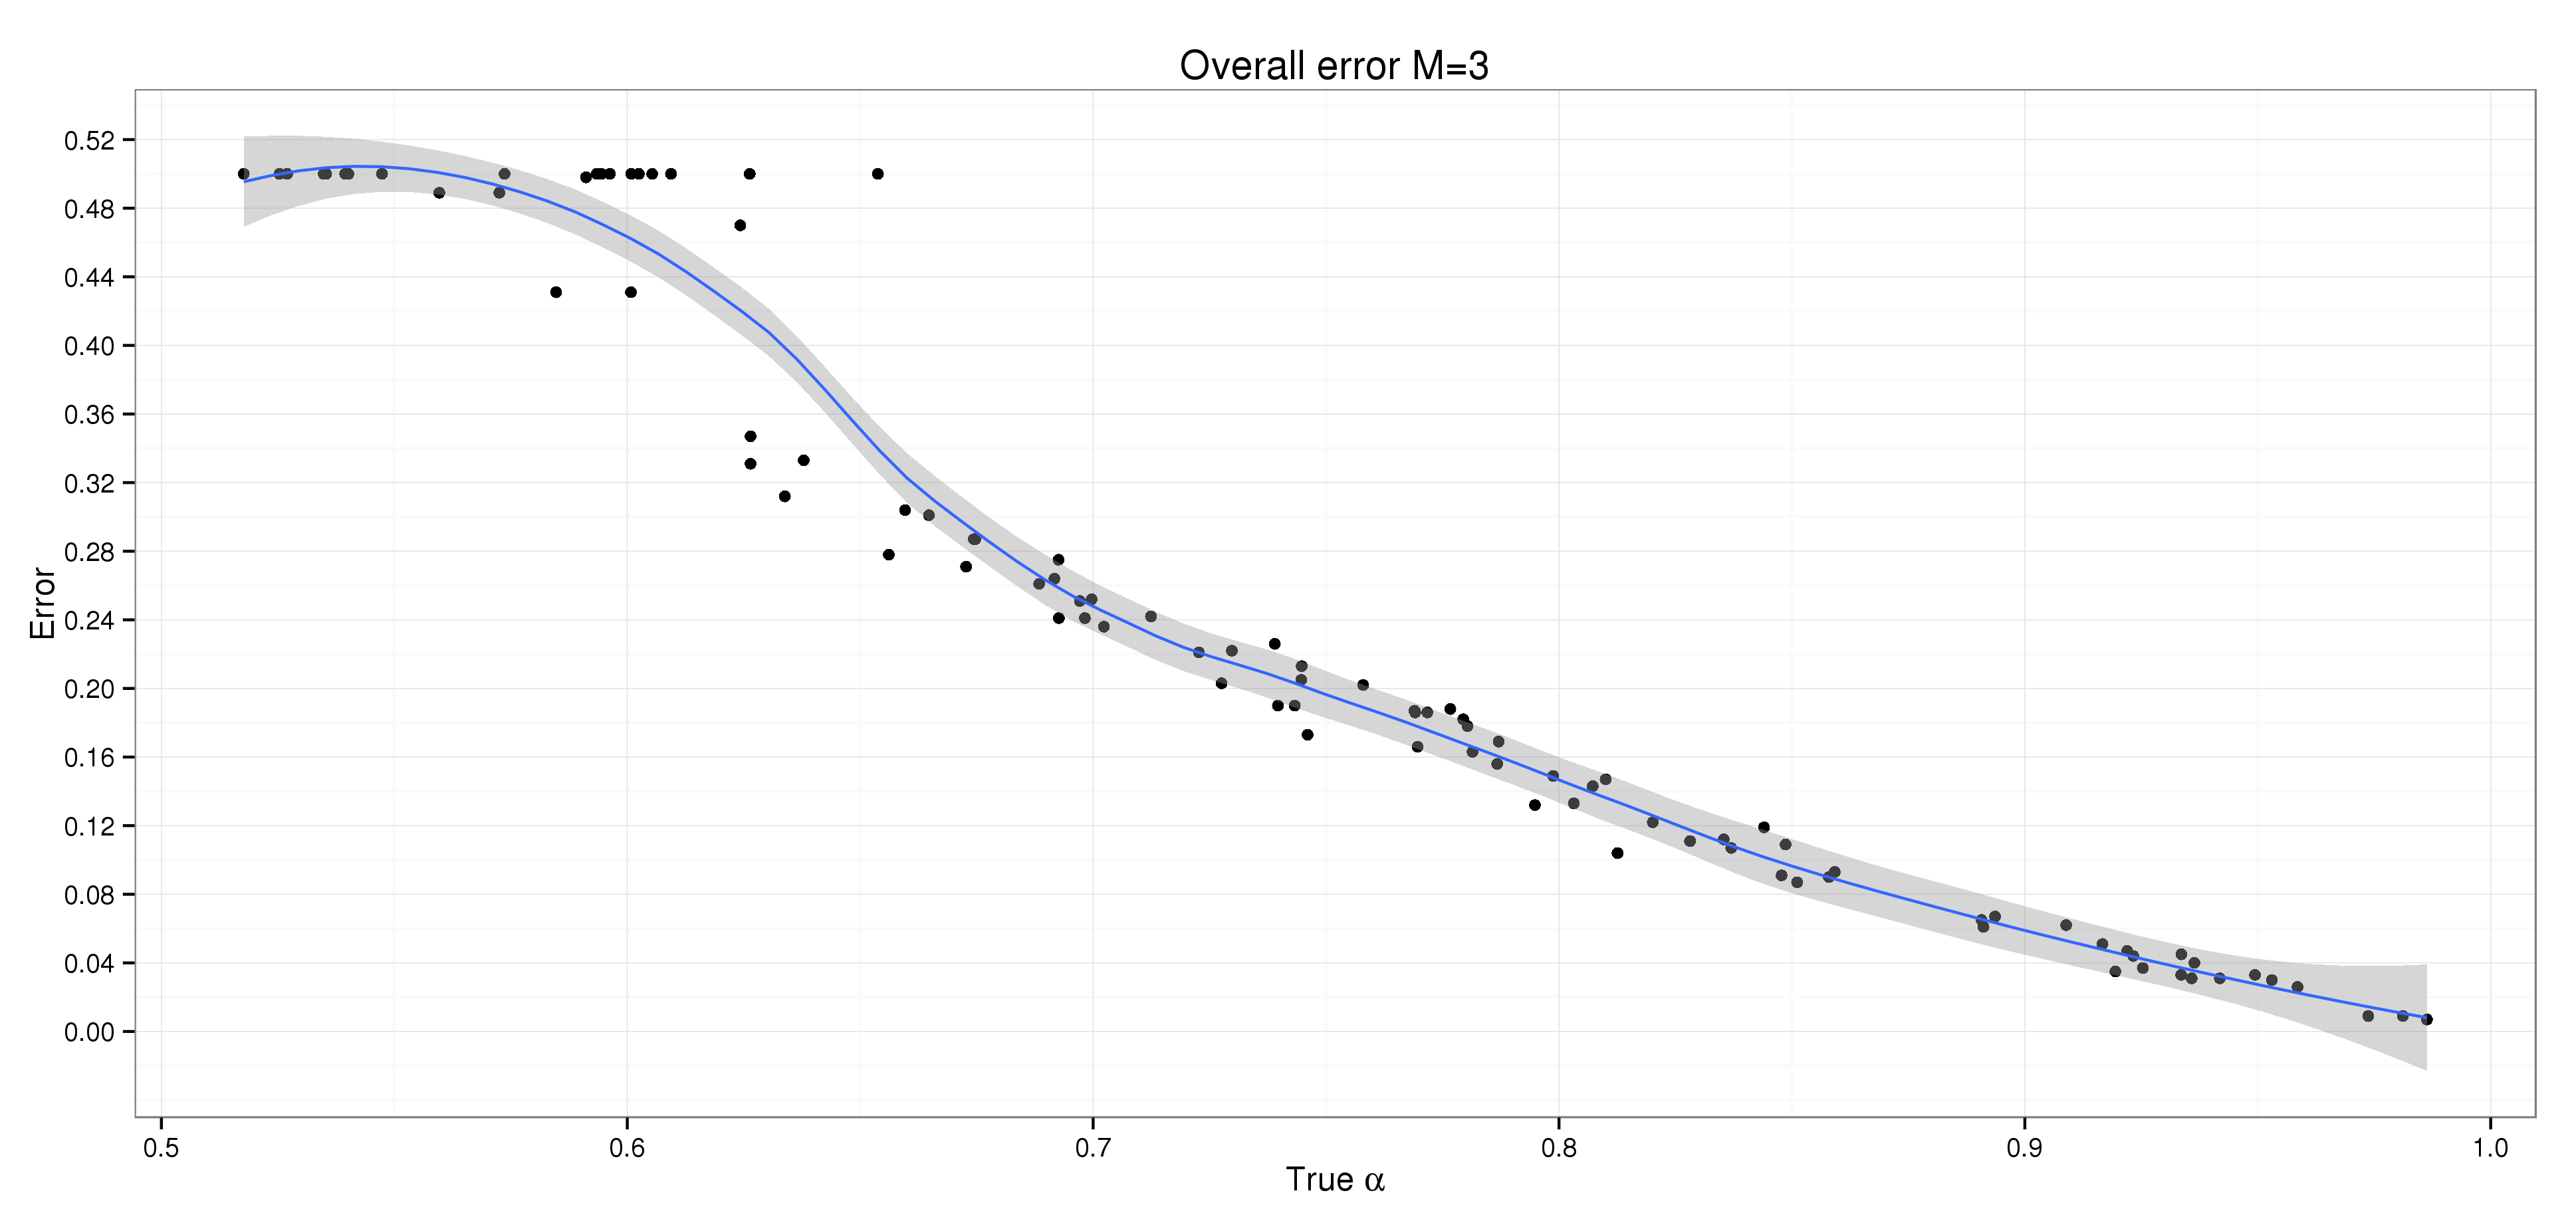
\includegraphics[scale = 0.39]{images/overallError.png}
\caption{\emph{Overral clustering error as a function of $\alpha$ for 100 realizations with $M=3$ data sources and $K=2$ clusters.}}
\label{overall-error-pic}
\end{center}
\end{figure}

Both, $\mathbf{L}_{error}$ and $\mathbf{C}_{error}$ decrease as the value of $\alpha$ increases, and they almost reach 0, when $\alpha \approx 1$. Both of these results confirm, in a different view, the results shown in \emph{Fig. \ref{adherence-test-pic}}, since the lower the error, the more accurate the estimates for the value of $\alpha$.

\citet{Lock2013} performed further analysis on the clustering accuracy by comparing the BCC model with separate clustering, joint clustering and dependent clustering, where they showed that BCC can be seen as a flexible bridge between the extremes of separate and joint clusterings.